\begin{frame}{$\Underset{\only<2->{\color{red}\check{C}ech}}{\text{\sout<2->{Sheaf}}}$ cohomology}
	Hence:
	\begin{center}
	\bfseries
		(pre)sheaves mediate the passage from local to global.
	\end{center}

	Most importantly, they enable the right tooling to study obstructions to this passage, namely \textbf{$\Underset{\only<2->{\color{red}\check{C}ech}}{\text{\sout<2->{sheaf}}}$ cohomology}.

	\vfill

	\onslide<3->{
		Reasons to prefer \v{C}ech to plain cohomology:
		\begin{enumerate}
			\item It's computational \setnote{(it's a simplicial cohomology in disguise)}
			\item Easily generalized to non-abelian sheaves (e.g. $\Set$-sheaves)\\
		\end{enumerate}
		For this talk though, let's stick to the \emph{abelian} version, hence we will assume \emph{$F$ is a sheaf valued in $\Ab$} \setnote{(or any abelian cat if you know what that means)}
	}
\end{frame}

\begin{frame}{\v{C}ech cohomology}
	Take a `good' cover $\{U_i\}_{i \in I}$ of $X$. \setnote{(e.g. contractible intersections)}
	\vfill
	Consider the following \textbf{chain complex}: \setnote{(meaning $\im d_n \subseteq \ker d_{n+1}$)}
	\begin{diagram*}
		0 \arrow{r} \&[-6ex] \prod_i F(U_i) \arrow{r}{d_0} \&[-5ex] \prod_{i,j} F(U_i \cap U_j) \arrow{r}{d_1} \&[-5ex] \prod_{i,j,k} F(U_i \cap U_j \cap U_k) \arrow{r}{d_2} \&[-5ex] \cdots
	\end{diagram*}
	where
	\begin{eqalign*}
		d_0((s_i)_i) &= (s_i \vert_{U_i \cap U_j} - s_j \vert_{U_i \cap U_j})_{i,j}\\
		d_1((s_{i,j})_{i,j}) &= (s_{i,j}\vert_{U_i \cap U_j \cap U_k} - s_{j,k}\vert_{U_i \cap U_j \cap U_k} + s_{k,i}\vert_{U_i \cap U_j \cap U_k})_{i,j,k}
	\end{eqalign*}
	and so on...
	\vfill
\end{frame}

\begin{frame}{\v{C}ech cohomology}
	The cohomology of the complex measures how far is $\im d_n$ from coinciding with $\ker d_{n+1}$: \setnote{('exactness')}
	\begin{diagram*}
		0 \arrow{r} \&[-6ex] \prod_i F(U_i) \arrow[squiggly, colornote]{d} \arrow{r}{d_0} \&[-5ex] \prod_{i,j} F(U_i \cap U_j) \arrow[squiggly, colornote]{d} \arrow{r}{d_1} \&[-5ex] \prod_{i,j,k} F(U_i \cap U_j \cap U_k) \arrow[squiggly, colornote]{d} \arrow{r}{d_2} \&[-5ex] \cdots\\[-5ex]
		\& H^0 = \ker d_0 \& H^1 = \dfrac{\ker d_1}{\im d_0} \& H^2 = \dfrac{\ker d_2}{\im d_1}
	\end{diagram*}
	\onslide<2->{
		Meaning:
		\begin{eqalign*}
			H^0 &= \text{local sections $(s_i)_i$ s.t. $s_i\vert_{U_i \cap U_j} = s_j\vert_{U_i \cap U_j}$ $\forall i,j \in I$}\\
			&\overset{\text{glueing}}= \text{\color{red}global sections}.\\
			H^1 &= \text{compatible local sections on $U_i \cap U_j$}\\
			&\phantom{=}\ \ \text{which do not arise from an assignment on the opens}\\
			&\approx \text{\color{red}$1$-holes}\\
			H^n &= \cdots \approx \text{\color{red}$n$-holes}
		\end{eqalign*}
	}
\end{frame}

\begin{frame}{\v{C}ech cohomology: example}
	\vspace{1ex}
	\begin{minipage}[b]{\textwidth}
		\begin{minipage}{.4\textwidth}
			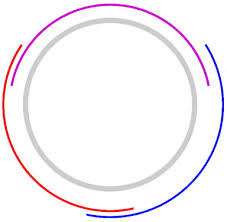
\includegraphics[width=.6\columnwidth]{figures/s1_cover.png}
		\end{minipage}%
		\begin{minipage}{.6\textwidth}
			Cover $S^1$ as in the picture,\\let $F =$ constant sheaf at $K$ field.
			\begin{diagram*}
				\text{\v{C}ech complex:} \quad 0 \arrow{r} \&[-5ex] K^3 \arrow{r}{d_0} \&[-5ex] K^3 \arrow{r}{d_1} \&[-5ex] 0
			\end{diagram*}
		\end{minipage}
	\end{minipage}
	\vspace{1ex}
	\onslide<2->{
		\begin{eqalign*}
			d_0 &= \begin{pmatrix}
				1 & -1 & 0\\
				0 & 1 & -1\\
				-1 & 0 & 1
			\end{pmatrix}\onslide<3->{\implies \operatorname{rk}(d_0) = 2 \implies \!\begin{cases}
				\dim \ker d_0 = 1,\\
				\dim \im d_0 = 2
			\end{cases}}\\[2ex]
			\onslide<4->{d_1 &= 0} \phantom{xxxxxxxxxxxxxxxxxxxxxxxxxxxxxx}\; \onslide<5->{\implies \dim \ker d_1= 3}\\
		\end{eqalign*}
	}
	\onslide<6->{
		Hence
		\vspace{-3ex}
		\begin{center}
			\begin{minipage}{.4\textwidth}
				\begin{eqalign*}
					H^{\color{blue}0} &= K^{\color{red}1}\\
					H^{\color{blue}1} &\iso K^3/K^2 \iso K^{\color{red} 1}\\
					H^{\color{blue}n} &= 0 \iso K^{\color{red}0}
				\end{eqalign*}%
			\end{minipage}%
			\begin{minipage}{.45\textwidth}%
				\begin{eqalign*}
					&\text{{\color{red}1} {\color{blue}0}-hole = 1 connected component}\\
					&\text{{\color{red}1} {\color{blue}1}-hole}\\
					&\text{{\color{red}0} {\color{blue}n}-holes for all $n \geq 2$}
				\end{eqalign*}
			\end{minipage}
		\end{center}
	}
\end{frame}

\begin{frame}{\v{C}ech cohomology}
	Cohomology is not completely determined by the topology of the space though, it is really determined by the structure of the sheaf \setnote{(it's the cohomology of its étalé space)}.
	\vfill
	\begin{example}
		\vspace{1.5ex}
		\begin{minipage}{.2\textwidth}
			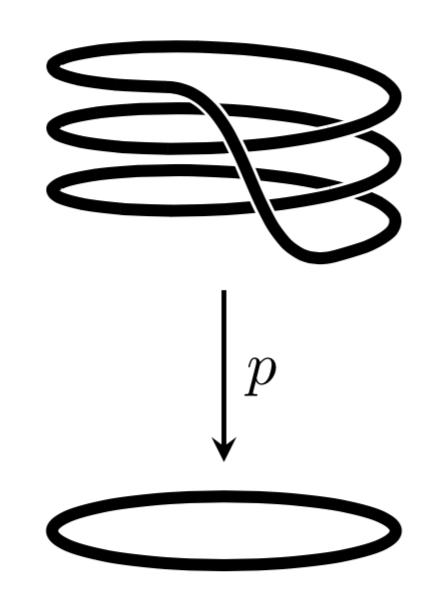
\includegraphics[width=.8\columnwidth]{figures/s1_triple_covering.png}
		\end{minipage}
		\begin{minipage}{.7\textwidth}
			Repeat the previous computation with a different \emph{locally} constant sheaf.
		\end{minipage}
	\end{example}
	\vfill
	Hence \textbf{topological obstructions $\neq$ local-to-global obstructions}!
\end{frame}

\begin{frame}{\v{C}ech cohomology: systems theory}
	% In terms of systems theory, \textbf{cohomology detects generative effects}.
	% \vfill
	Let $B$ {\color{colornote}(presheaf of behaviours)} be a \textbf{pre}sheaf of abelian groups, let $\{U_i\}_{i \in I}$ open covering of $U$.

	Its \textbf{{\color{red}{augmented}} \v{C}ech complex} is:
	\begin{diagram*}
		0 \arrow{r} \&[-5ex] \color{red}{B(U)} \arrow[visible on=<2->, squiggly, colornote]{d} \arrow[red]{r}{d_{-1}} \&[-5ex] \prod_i B(U_i) \arrow[visible on=<2->, squiggly, colornote]{d} \arrow{r}{d_0} \&[-5ex] \prod_{i,j} B(U_i \cap U_j) \arrow[visible on=<2->, squiggly, colornote]{d} \arrow{r}{d_1} \&[-5ex] \cdots\\[-5ex]
		\&[-5ex] \onslide*<2->{\color{blue}{H^{-1} = \ker d_{-1}}} \& \onslide*<2->{\color{blue}{H^0 = \dfrac{\ker d_0}{\im d_{-1}}}} \& \onslide*<2->{H^1 = \dfrac{\ker d_1}{\im d_0}} \& \onslide*<2->{\cdots}
	\end{diagram*}
	where {\color{red}$d_{-1}(s) = (s\vert_{U_i})_i$}.
	\begin{eqalign*}
		\onslide<3->{H^{-1} &= \text{failure of $B$ to be separated \color{colornote}{($=0$ iff separation holds)}}}\\
		&\qquad\onslide<6->{\rightsquigarrow \text{\color{red}\bfseries interactive behaviour}}\\
		\onslide<4->{H^0 &= \text{failure of $B$ to glue \color{colornote}{($=0$ iff glueing holds)}}}\\
		&\qquad\onslide<6->{\rightsquigarrow \text{\color{red}\textbf{emergent behaviour} (Adam, 2017)}}\\
		\onslide<5->{H^{\geq 1} &= \text{same as before!}}\onslide<7->{\rightsquigarrow \text{\bfseries higher-order emergent behaviour...?}}\\
	\end{eqalign*}
\end{frame}
